\documentclass{article}
% WIP!
% Based upon: https://glennjlea.com/latex/creating-custom-title-page/
\usepackage{bootstrapcolors}
\usepackage{tikz}
\usetikzlibrary{arrows,shapes.gates.logic.US,shapes.gates.logic.IEC,calc}
\begin{document}
    \color{orange-400}
    \pagecolor{blue-800}
    \thispagestyle{empty}
    \begin{center}
        \tikzstyle{branch}=[fill,shape=circle,minimum size=3pt,inner sep=0pt]
        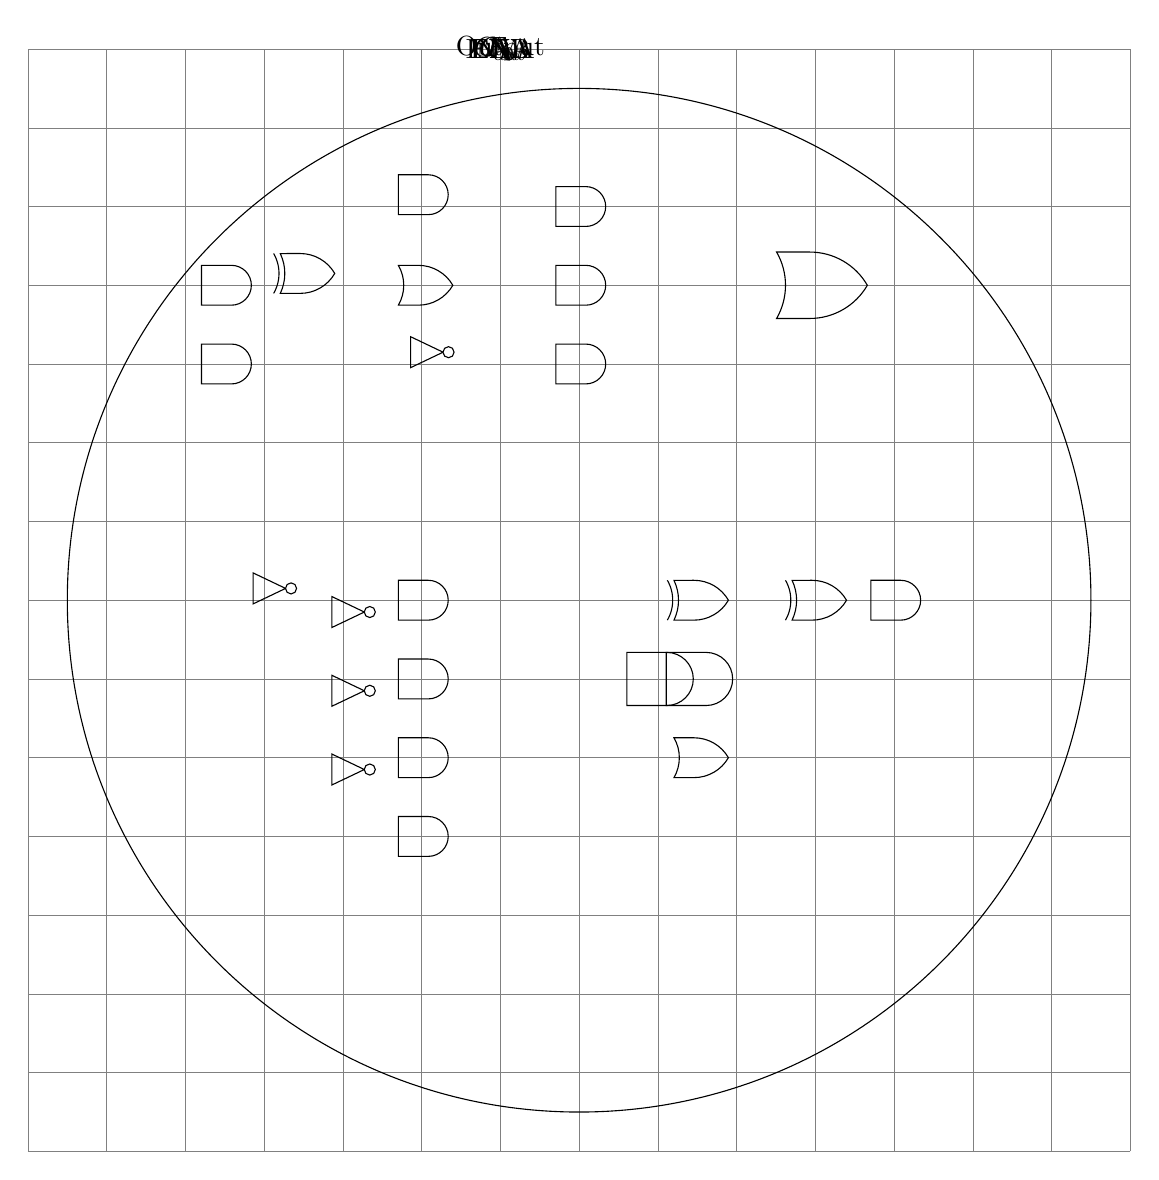
\begin{tikzpicture}
            % 1-bit ALU
            \draw[help lines] (-7,7) grid (7,-7); % Only for Development
            %\node (a) at (-3,7) {$a$};
            %\node (b) at (-2,7) {$b$};
            %\node (c) at (-1,7) {$c$};
            
            \node (inva) at (-1,7) {INVA};
            \node (a) at (-1,7) {A};
            \node (b) at (-1,7) {B};
            \node (ena) at (-1,7) {ENA};
            \node (enb) at (-1,7) {ENB};
            \node (f0) at (-1,7) {$F_0$};
            \node (f1) at (-1,7) {$F_1$};
            \node (cin) at (-1,7) {$C_{in}$};
            \node (cout) at (-1,7) {$C_{out}$};
            \node (output) at (-1,7) {Output};
            
            \node[and gate US, draw, logic gate inputs=nn] at (0,5) (AND1) {};
            \node[and gate US, draw, logic gate inputs=nn] at (0,4) (AND2) {};
            \node[and gate US, draw, logic gate inputs=nn] at (0,3) (AND3) {};
            
            \node[and gate US, draw, logic gate inputs=nn] at (-2,5.15) (AND4) {};
            \node[or gate US, draw, logic gate inputs=nn] at (-2,4) (OR1) {};
            \node[not gate US, draw, logic gate inputs=n] at (-2,3.15) (NOT1) {};
            
            \node[xor gate US, draw, logic gate inputs=nn] at (-3.5,4.15) (XOR1) {};
            \node[and gate US, draw, logic gate inputs=nn] at (-4.5,4) (AND5) {};
            \node[and gate US, draw, logic gate inputs=nn] at (-4.5,3) (AND6) {};
            
            \node[or gate US, draw, logic gate inputs=nnnn] at (3,4) (OR2) {};

            \node[and gate US, draw, logic gate inputs=nn] at (-2,0) (AND7) {};
            \node[and gate US, draw, logic gate inputs=nn] at (-2,-1) (AND8) {};
            \node[and gate US, draw, logic gate inputs=nn] at (-2,-2) (AND9) {};
            \node[and gate US, draw, logic gate inputs=nn] at (-2,-3) (AND10) {};

            \node[not gate US, draw, logic gate inputs=n] at (-3,-0.15) (NOT2) {};
            \node[not gate US, draw, logic gate inputs=n] at (-3,-1.15) (NOT3) {};
            \node[not gate US, draw, logic gate inputs=n] at (-3,-2.15) (NOT4) {};
            
            \node[not gate US, draw, logic gate inputs=n] at (-4,0.15) (NOT5) {};
            
            \node[xor gate US, draw, logic gate inputs=nn] at (1.5,0) (XOR2) {};
            \node[xor gate US, draw, logic gate inputs=nn] at (3,0) (XOR3) {};
            \node[and gate US, draw, logic gate inputs=nn] at (4,0) (AND11) {};
            
            \node[and gate US, draw, logic gate inputs=nnn] at (1,-1) (AND12) {};
            \node[and gate US, draw, logic gate inputs=nnn] at (1.5,-1) (AND13) {};
            \node[or gate US, draw, logic gate inputs=nn] at (1.5,-2) (OR3) {};

            %\draw (a.south) -- ++(south:0mm) |- (GOR.input 1);
            %\draw (GOR.output) -- ++(right:3mm);

            \draw (0,0) circle [radius=6.5];
        \end{tikzpicture}
    \end{center}
\end{document}